\documentclass[deposito, acronym, symbols]{fei}

%\usepackage{glossaries}
\usepackage{subcaption} 
\usepackage{graphicx}
\usepackage{float}
%\usepackage{units}
\usepackage[portuguese]{algorithm2e}
\usepackage{biblatex}
\usepackage{amsmath}
\usepackage{listings}
\usepackage[utf8]{inputenc}
\usepackage{chngcntr} %Faz com que o numero das notas de rodape aumente crescentemente.
\usepackage{appendix}
\counterwithout{footnote}{chapter}% "
\usepackage{siunitx}
\sisetup{output-exponent-marker=\ensuremath{\mathrm{e}}} %Escrita que precede cada entrada na lista de ilustrações.
\renewcommand{\cftfigurepresnum}{Figura }
\setlength{\cftfigurenumwidth}{5.7em}

\usepackage{titling}

%\makeglossaries
%%\newacronym[] {achpt} {ACT} {Aparecido ChupeTão}

\newacronym[longplural=Associações Brasileiras de Normas Técnicas]{abnt}{ABNT}{Associação Brasileira de Normas Técnicas}

\newacronym{ibge}{IBGE}{Instituto Brasileiro de Geografia e Estatística}

\newacronym{ashrae}{ASHRAE}{\textit{American Society of Heating, Refrigerating and Air-Conditioning Engineers}}

\newacronym{nbr}{NBR}{Norma Brasileira}

\newacronym{pmv}{PMV}{\textit{Predicted Mean Vote}}
	
\newacronym{ppd}{PPD}{\textit{Predicted Percentage of Dissatisfied}}
		
\newacronym{vgd}{VGD}{Ventilação Geral Diluidor}
		
\newacronym{vgl}{VGL}{Ventilação Local Exaustora}
		
\newacronym{cfd}{CFD}{\textit{Computational Fluid Dynamics}}
		
\newacronym{pcb}{PCB}{\textit{Printed Circuit Board}}
		
\newacronym{sms}{SMS}{\textit{Short Message Service}}
		
%\newglossaryentry{pi}{parent=greek,type=symbols,name={\ensuremath{\pi}},sort=p,description={número irracional que representa [razão entre a circunferência de qualquer círculo e seu diâmetro]}}
		


\title{ESFORÇOS NO TORNEAMENTO - LEVANTAMENTO DO Ks1 - Grupo C}
\author{ Felipe Estevão Coquito de Mello - 11.120.486-3 \\ Gabriel Mola da Silva - 11.120.255-2 \\ Netuno Trindade Torrente Rovaroto - 11.120.321-2 \\ Diurno - Vitoria Fedatto Stefaneli - 11.120.497-0}
\cidade{São Bernardo do Campo}
\instituicao{Centro Universitário FEI}

\addbibresource{Referencias.bib}
%\bibliographystyle{plain}
\bibliography{Referencias}
\graphicspath{ {Imagens/}, {Tabelas/}}

\begin{document}
\maketitle

\begin{folhaderosto}
	Relatório apresentado ao departamento de Engenharia Mecânica do Centro Universitário FEI, como parte dos requisitos de avaliação da disciplina ME140 – Usinagem. Solicitado pelo Prof. Adalto de Farias.
\end{folhaderosto}

\begin{resumo}

Como em toda usinagem existem alguns parâmetros que influenciam e afetam o resultado final da peça, tais como a velocidade de avanço, a rotação do torno, o avanço e a profundidade de corte. O objetivo deste relatório é realizar o levantamento experimental dos valores de $Ks_1$ (pressão específica de corte unitária) e de z da equação de Kienzle e estudar a influência dos parâmetros de usinagem na rugosidade da peça acabada. Para isso, um experimento alterando a rotação do torno, o avanço e a profundidade de corte da máquina, com quinze diferentes combinações dos parâmetros foi realizado no laboratório, a fim de esclarecer como tais parâmetros afetam a pressão específica de corte. Após isso, as rugosidades de cada experimento com as diferentes especificações do torno foram medidas. Os resultados experimentais foram comparados com a literatura e pode-se dizer que foram ligeiramente diferentes. Foi possível observar que o avanço e a profundidade de corte têm grande influência na rugosidade final das peças, nas forças de usinagem e, consequentemente, na pressão específica de corte. 

\palavraschave{Pressão específica de corte. Rugosidade. Kienzle.}

\end{resumo}

\tableofcontents
\listoffigures
\listoftables

\chapter{Introdução}
O estudo de processos de usinagem consistem em verificar como vários fatore afetam a peça final. Fatores esses como o desgaste da ferramenta, as características do material da peça e da ferramenta, a temperatura e o calor gerado durante o processo de corte. 

No processo de corte do metal, há a ação de forças de usinagem e, consequentemente, há uma pressão específica de corte. Tais componentes são medidos através de experimentos em que se mudam a velocidade de corte, o avanço, a rotação do torno mecânico e a profundidade de corte. Ao mudar tais parâmetros muda-se também a rugosidade do material, afetando diretamente a qualidade, a eficiência e a economia de um processo de fabricação, determinando custos de operação e preço final da peça. 

Deste modo, será desenvolvida neste relatório uma análise mais aprofundada de como tais variáveis ditam o comportamento da força de corte, da pressão específica de corte e da rugosidade. 

\section{Problemas e motivações para o estudo}

Diversos problemas podem surgir caso a força de corte, a pressão específica de corte e a rugosidade não sejam estudadas de forma assertivas. Entre os diversos problemas, podem-se citar:  má qualidade da peça, desperdício de material, desgaste excessivo da ferramenta, aumento do tempo de produção, aumento dos custos, além de adquirir uma rugosidade inadequada, resultando em uma peça com superfícies ásperas ou irregulares, o que leva à insatisfação dos clientes. 

\section{Objetivos do trabalho}

O objetivo deste relatório é realizar, através de experimentos realizados em laboratório, o levantamento  dos valores da pressão específica de corte unitário ($Ks_1$) e de z da equação de Kienzle e estudar a influência dos parâmetros de usinagem na rugosidade da peça acabada. 

Para os experimentos foi utilizado um material com características conhecidas (aço ABNT 1045) avaliando como a mudanças dos parâmetros afetaram a força de corte e a rugosidade do metal.

\chapter{Referencial teórico}

\section{Forças de usinagem}

Segundo, \textcite{machado2015teoria},  %( <= Isso é igual a isso Machado et al.)
o conhecimento da força de usinagem e de suas componentes é de grande importância para o estudo do processo de usinagem, pois deste modo é possível estimar a potência de corte e as forças atuantes na máquina, viabilizando, assim um menor desgaste desta e uma maior economia no processo. 
A Figura \ref{fig: Forças de usinagem} mostra como essa força é decomposta em suas três principais componentes, sendo elas a força de corte ($F_c$), a força de avanço ($F_f$) e a força passiva ou de penetração ($F_p$).

\begin{figure}[!htb]
 \centering
    \caption{Forças de usinagem}
    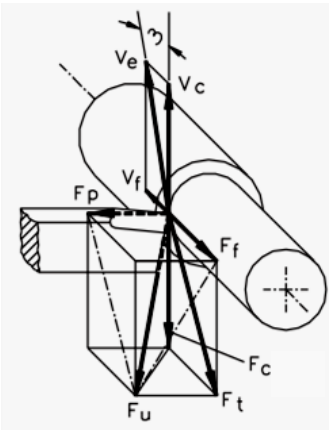
\includegraphics[width=0.4\linewidth]{Imagens/Forças de usinagem (1).png}
    \smallcaption{Fonte: \textcite{machado2015teoria}}
    \label{fig: Forças de usinagem}
 \end{figure}
 
As componentes da força de usinagem são:

Força de corte ($F_c$): é a projeção da força de usinagem no plano de trabalho, no sentido do corte;

Força de avanço ($F_f$): é a força dada na direção do avanço e projetada no plano de trabalho;

Força passiva ou de penetração ($F_p$): é a força de usinagem projetada perpendicularmente ao plano de trabalho em direção ao avanço.

A força de usinagem é sempre decomposta em suas três componentes, portanto vale a representação matemática:

\begin{equation}
    Fu=\sqrt{F_c^2+F_f^2+F_p^2}    
    \label{eq: Força de usinagem}
\end{equation}
 

\section{Força de corte}
A força de corte, uma das principais componentes para determinação da potência de usinagem, é a mais afetada pela seção do cavaco. Essa relação seção de cavaco - força de corte é praticamente linear e, portanto, foi proposta, por cientistas do século XX, uma equação para determinar a força de corte teórica no processo de usinagem. A equação (\ref{eq: Força de corte teórica}) mostra a proposta.

\begin{equation}
    F_c=Ks\times{A}  
    \label{eq: Força de corte teórica}
\end{equation}

\begin{equation}  
    A=h\times{b}
    \label{eq: Área da seção de corte}
\end{equation}

\begin{equation}
    h=fn\times{sen(Kr)}
    \label{eq: Fórmula do h}
\end{equation}

\begin{equation}
    b=\frac{a_p}{sen(Kr)}
    \label{eq: Fórmula do h_2}
\end{equation}



Onde $Ks$ é chamado de pressão específica de corte e $A$ é a área da seção de corte do cavaco, sendo $h$ a espessura e $b$ o comprimento ativo do cavaco. $Kr$ é o ângulo da ferramenta, $fn$ é o avanço e $a_p$ é a profundidade de corte. A Figura \ref{fig: Força de corte} ilustra como é medida a força de corte.

\begin{figure}[!htb]
 \centering
    \caption{Força de corte}
    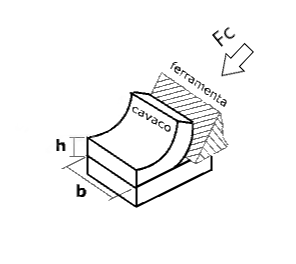
\includegraphics[width=0.5\linewidth]{Imagens/força de corte 1.png}
    \smallcaption{Fonte: Adaptado de \textcite{peixoto2013analise}}
    \label{fig: Força de corte}
 \end{figure}

 
Alguns fatores podem influenciar a $F_c$, como o material da peça, pois quanto maior a resistência do material, maior será a dificuldade de cisalhá-lo, aumentando assim a força de usinagem. Outro fator que influencia a $F_c$ é o material da ferramenta que depende da afinidade química entre a ferramenta e o material da peça, podendo aumentar ou diminuir o esforço de corte. Ainda sobre a ferramenta, a geometria desta também tem influência sobre a força de corte e o ângulo de saída da ferramenta é o mais influente, isto porque, quanto menor o ângulo de saída maior será a área de contato ferramenta-peça e portanto aumentará a força de corte. E, por fim, o uso ou não de fluido de corte. Se utilizar o fluido de corte, este diminuirá a área de contato do cavaco com a ferramenta e, por conseguinte, diminuirá a força de corte.



 \section{Pressão específica de corte}
 
A pressão específica de corte já foi muito pesquisada, porém as pesquisas mostram que a pressão teórica difere muito daquela vista em laboratório, portanto foi decido que cada par ferramenta/peça, com certos valores de parâmetros de usinagem, terá sua própria pressão específica de corte. Ela é uma relação entre a força de corte ($F_c$) e a área da seção do cavaco, como mostrado na equação (\ref{eq: Pressão específica de corte}). Com a área da seção do cavaco sendo calculada da mesma forma que a equação (\ref{eq: Área da seção de corte}). 


\begin{equation}
    Ks=\frac{F_c}{A}
    \label{eq: Pressão específica de corte}
\end{equation}



Entre todos os modelos desenvolvidos para o cálculo do $Ks$ o que mais se destaca é o de Kienzle que deduziu uma expressão simples (equação (\ref{eq: Fórmula do Ks})), porém bem precisa para a correção da pressão específica de corte ($Ks$), de acordo com a espessura do cavaco ($h$). Os valores de $Ks_1$ e $z$ são achados experimentalmente para cada par ferramenta/peça com uma combinação prévia de certos parâmetros de usinagem. 


\begin{equation}
    Ks=Ks_1\times{h^{-z}}
    \label{eq: Fórmula do Ks}
\end{equation}

Kienzle também deduziu uma relação para achar a força de corte ($F_c$) utilizando o valore da pressão específica de corte unitária (equação (\ref{eq: Relação de Kienzle})).

\begin{equation}
    F_c=Ks_1\times{b}\times{h^{1-z}}
    \label{eq: Relação de Kienzle}
\end{equation}

Assim como a força de corte, alguns fatores influenciam a pressão específica de corte, sendo elas a dureza do material, o ângulo de saída da ferramenta e o uso ou não de fluido de corte.


\section{Rugosidade}

Segundo \textcite{machado2015teoria}, a rugosidade de uma superfície não é regular, ela pode ser composta por pequenas irregularidade resultantes da ação do processo de corte. A rugosidade é muito utilizada como um parâmetro de saída para controlar a condição e o processo de usinagem. Assim como a $F_c$ e o $Ks$ a rugosidade também é influenciada por vários parâmetros, sendo alguns deles: o material da peça a ser usinada, a geometria da ferramenta e a própria operação de usinagem.

Para medir a rugosidade da peça é necessário um aparelho chamado rugosímetro, que consiste em um aparelho com uma ponta de diamante que ao entrar em contato com a superfície da peça, começa a medir sua rugosidade em uma linha reta, previamente definida para a operação. 

Este aparelho, porém, têm algumas desvantagens como por exemplo a área de contato entre a ponta de diamante e a peça é muito pequena, gerando erros devido a pressão de contato muito elevada, causando danos em materiais macios e dificuldades em materiais com revestimento. Por outro lado, em materiais muito duros e abrasivos, os danos são na ponta do aparelho causando desgaste progressivo na máquina e deixando as análises cada vez menos fieis. A Figura \ref{fig:rugosimetro} mostra como é um rugosímetro.

\begin{figure}[!htp]
    \centering
    \caption{Rugosímetro}
    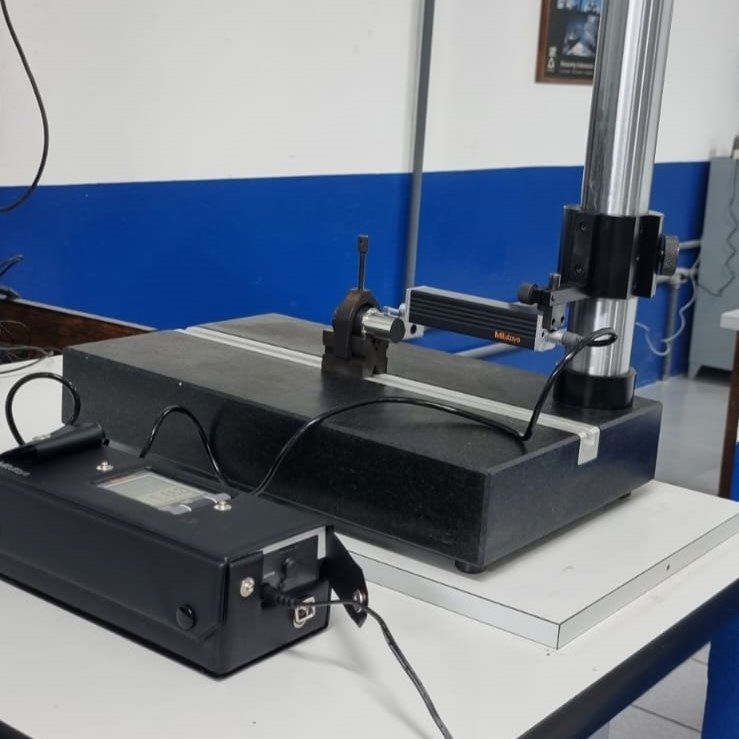
\includegraphics[width=0.6\linewidth]{Imagens/Exp01_rugosidade - Copia.jpeg}
    \smallcaption{Fonte: Autor}
    \label{fig:rugosimetro}
\end{figure}


\chapter{Metodologia}

O planejamento dos ensaios foi realizado em sala com o auxilio do técnico responsável pelo experimento, foi dividido em três partes como é possível ver na Tabela \ref{tab:Planejamento}. Sendo os primeiros ensaios com os valores de rotação ($n$) e a profundidade de corte ($a_p$) constantes e alterando a velocidade de avanço ($fn$), a segunda bateria de ensaios foi feita com os valores de $n$ e $fn$ constantes e os de $a_p$ variados e por fim $fn$ e $a_p$ constante e $n$ mudando. Com o objetivo de descobrir qual dessas variáveis interfere diretamente nos esforços e na rugosidade da peça.

\begin{table}[!htb]
 \centering
    \caption{Dados do experimento para aquisição de dados }
    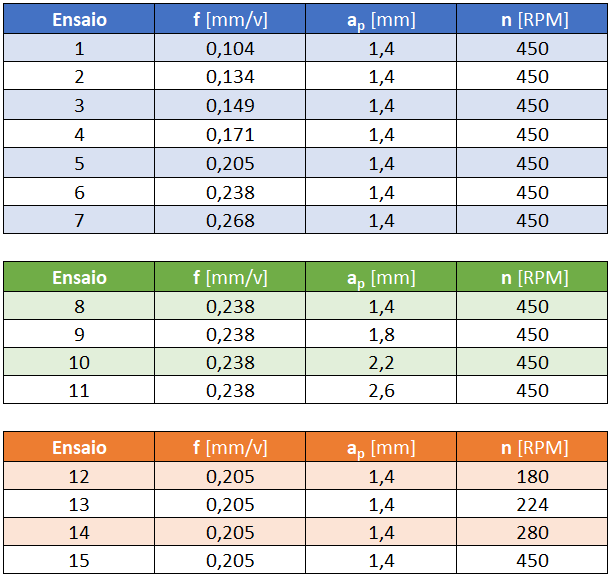
\includegraphics[width=0.85\linewidth]{Imagens/Exp01_planejamento.png}
    \smallcaption{Fonte: Autor}
    \label{tab:Planejamento}
 \end{table}

\section{Experimento}

O experimento foi realizado em um torno externo, Romi I 30A-A -10 cv, Figura \ref{fig:Torno} e utiliza o inserto SNMG 120408, Figura \ref{fig:fera}. O material que foi usinado foi uma barra de o Aço ABNT 1045, Figura \ref{fig:barra}  e a operação ocorreu à seco. O processo de obtenção dos dados foi dado pela sequência:

\begin{enumerate}
    \item Colocar os valores correspondeste de $n$ , $fn$ e $a_p$ do ensaio a ser executado no torno a partir da folha de Planejamento;
    \item Iniciar a operação de torneamento;
    \item Simultaneamente ao inicio da operação, começar a medição do esforço no software do computador;
    \item Finalizar a operação;
    \item Salvar os dados do ensaio, Figura \ref{fig:comp};
    \item Medir a rugosidade no rugosímetro, Figura \ref{fig:rugo}, e anotar o valor indicado;
    \item Repetir para próximo ensaio.
\end{enumerate}

\begin{figure}[!htp]
  \centering
  \begin{minipage}{0.4\textwidth}
    \centering
    \caption{Torno mecânico externo}
    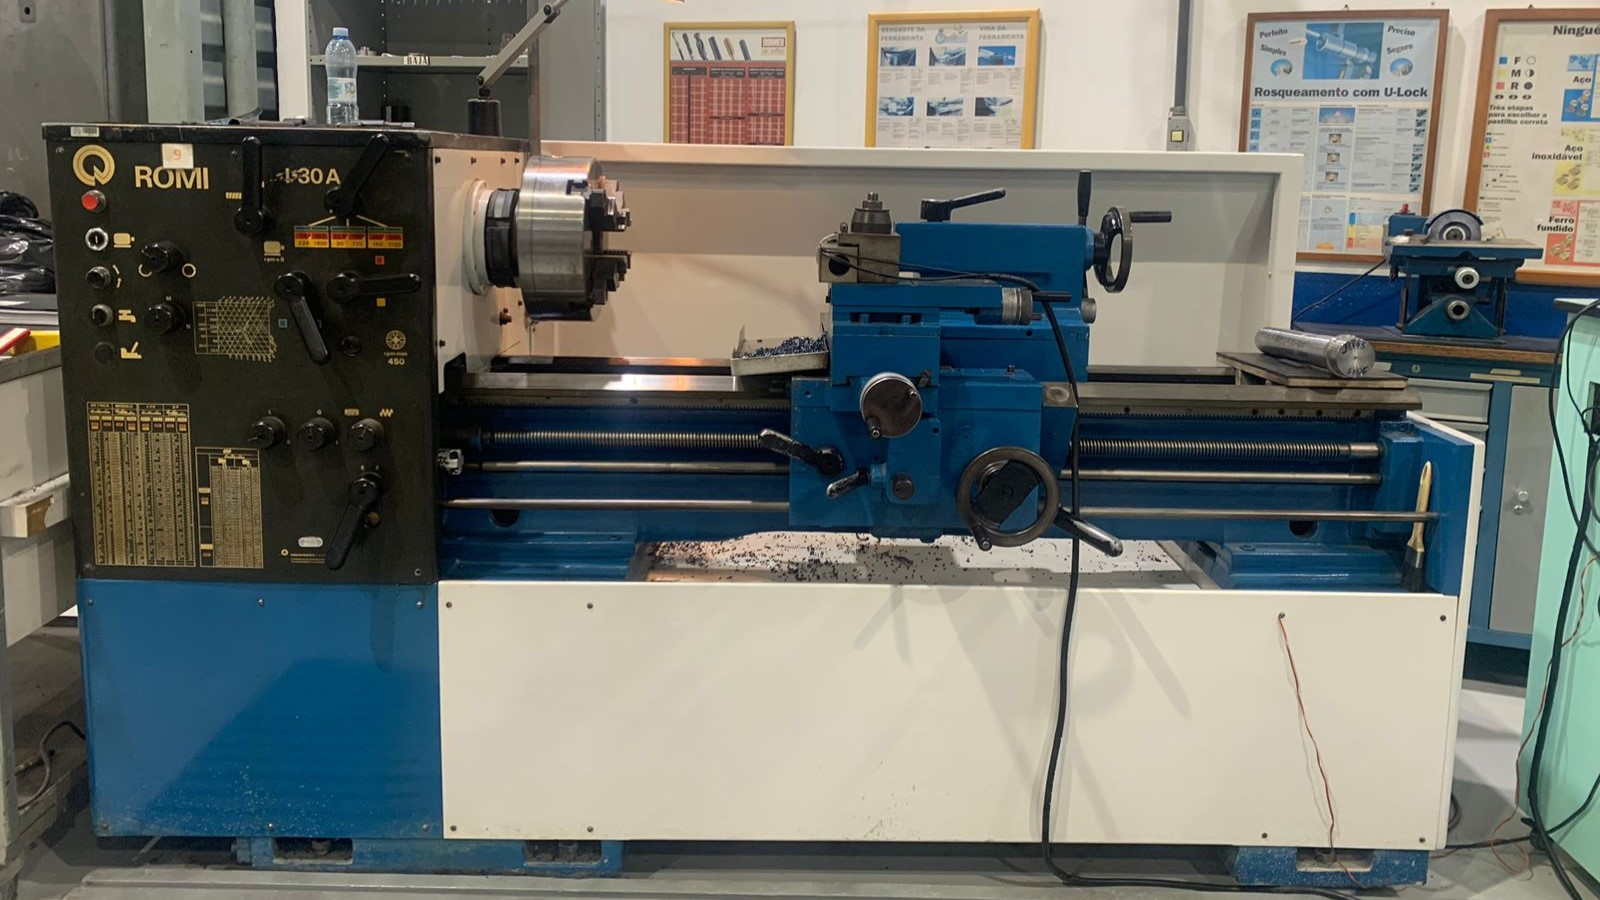
\includegraphics[width=1.1\linewidth]{Imagens/Exp01_torno.jpeg}
    \smallcaption{Fonte: Autor}
    \label{fig:Torno}
  \end{minipage}
  \hfill
  \begin{minipage}{0.4\textwidth}
        \caption{Ferramenta utilizada}
    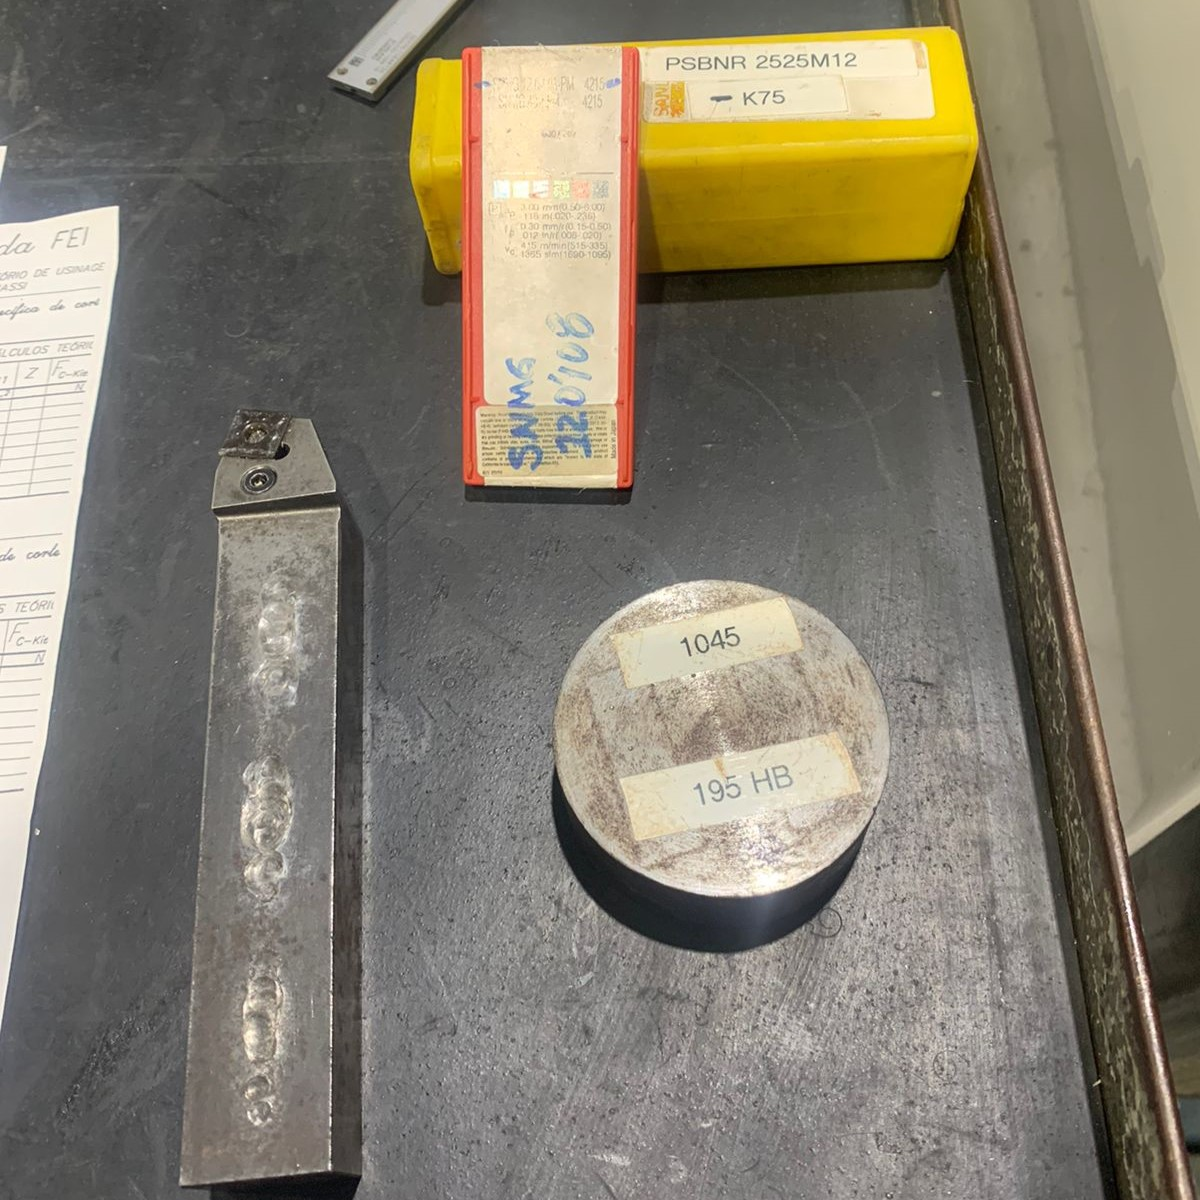
\includegraphics[width=0.8\linewidth]{Imagens/Exp01_ferramenta.jpeg}
    \smallcaption{Fonte: Autor}
    \label{fig:fera}
  \end{minipage}
\end{figure}


\begin{figure}[!htp]
    \centering
    \caption{Barra usinada em aula}
    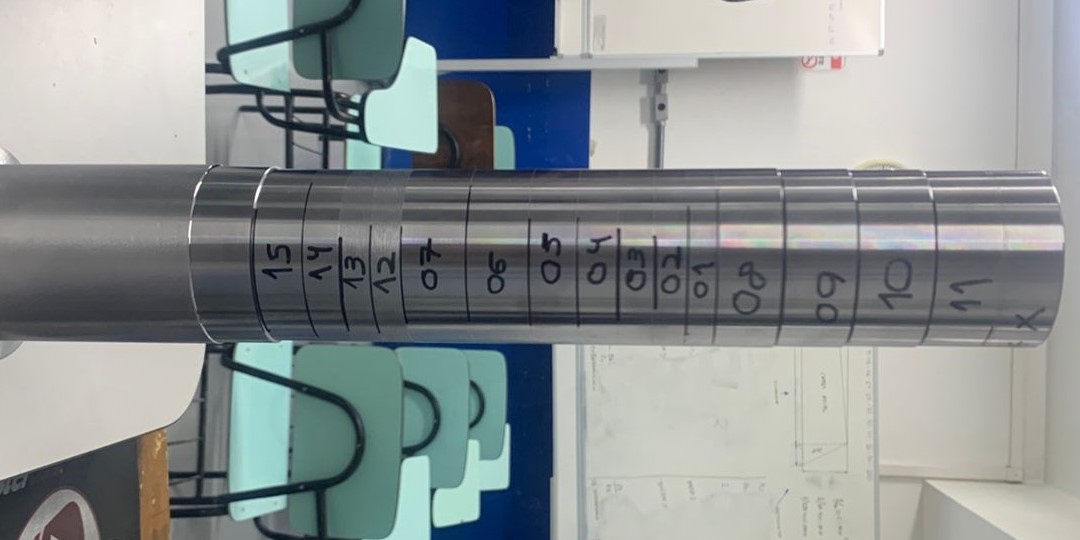
\includegraphics[width=0.6\linewidth]{Imagens/Exp01_barratorenada.jpeg}
    \smallcaption{Fonte: Autor}
    \label{fig:barra}
\end{figure}

\begin{figure}[!htp]
  \centering
  \begin{minipage}{0.4\textwidth}
    \centering
    \caption{Computador com software de medição de esforços}
    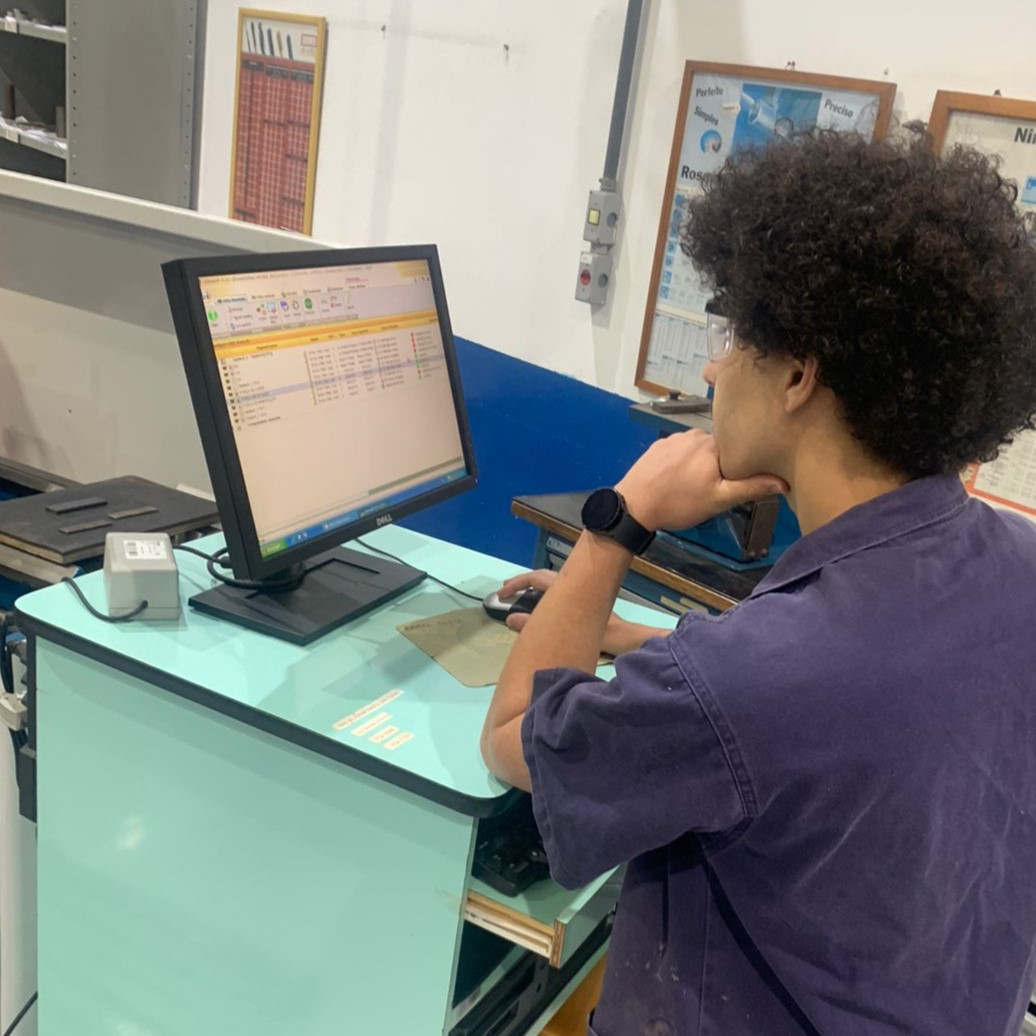
\includegraphics[width=1\linewidth]{Imagens/Exp01_computador.jpeg}
    \smallcaption{Fonte: Autor}
    \label{fig:comp}
  \end{minipage}
  \hfill
  \begin{minipage}{0.4\textwidth}
        \caption{Rugosímetro utilizado em aula}
    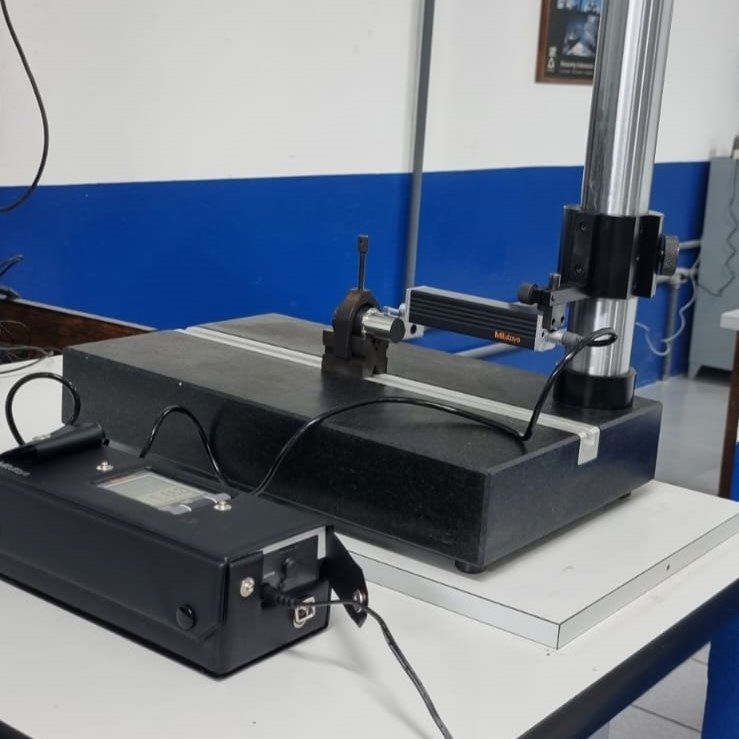
\includegraphics[width=1\linewidth]{Imagens/Exp01_rugosidade - Copia.jpeg}
    \smallcaption{Fonte: Autor}
    \label{fig:rugo}
  \end{minipage}
\end{figure}


\chapter{Resultados obtidos e discussões}

Com o objetivo citado em mente, certos parâmetros foram alterados para permitir uma análise mais aprofundada da influência dos parâmetros de usinagem na pressão específica e na rugosidade, visando saber quais deles afetaram mais os resultados. Nesse contexto, durante o experimento, foram ajustadas as seguintes variáveis: rotação ($n$), profundidade de corte ($a_p$) e avanço ($fn$). 



\section{Pressão específica de corte}

Para a coleta dos dados de pressão específica foram utilizados somente os sete primeiros experimentos, nos quais só foram alterados os avanços. Com os resultados de $F_c$ obtidos experimentalmente através do software e calculando a área da seção do cavaco através da equação (\ref{eq: Área da seção de corte}), foi possível, por meio da equação (\ref{eq: Fórmula do Ks}), calcular o valor da pressão específica de corte experimental ($Ks$ exp), como visto na Tabela (\ref{tab: parâmetros para ks}).  
A Tabela (\ref{tab: Adicional}) indicam os valores calculados para as variáveis $b$, $h$ e $A$, necessárias para os cálculos.

\begin{table}[!htb]
 \centering
    \caption{Parâmetros e resultados experimentais}
    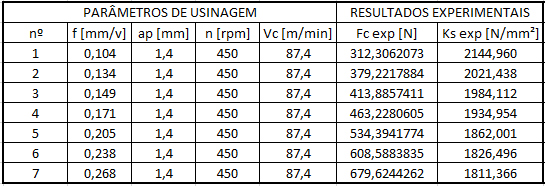
\includegraphics[width=0.85\linewidth]{Imagens/Tabela parâmetros e resultados ex.png}
    \smallcaption{Fonte: Autor}
    \label{tab: parâmetros para ks}
 \end{table}


\begin{table}[!htb]
 \centering
    \caption{Cálculos adicionais}
    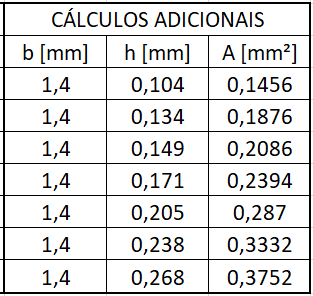
\includegraphics[width=0.3\linewidth]{Imagens/tabela calculos adic.png}
    \smallcaption{Fonte: Autor}
    \label{tab: Adicional}
 \end{table}
 
Com os parâmetros $Ks$ experimental e $h$  calculados, conseguiu-se traçar o gráfico (\ref{fig: grafico}) $Ks$ x $h$ e achar o $Ks_1$ experimental. Vale lembrar que a escala do gráfico, neste caso, é log-log.


\begin{figure}[!htp]
    \centering
    \caption{Gráfico experimental $Ks$ x $h$}
    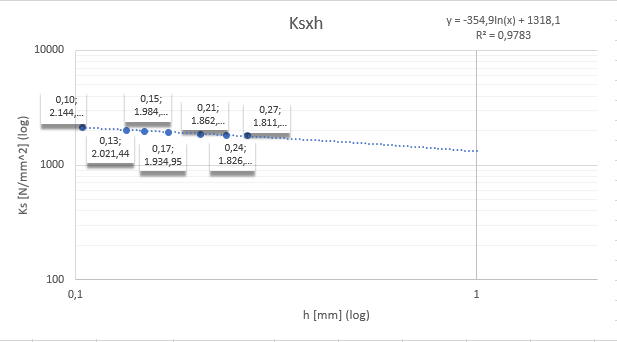
\includegraphics[width=0.6\linewidth]{Imagens/Gráfico Ksxh.png}
    \smallcaption{Fonte: Autor}
    \label{fig: grafico}
\end{figure}

 Os dados utilizados para fazer tal gráfico estão dispostos na Tabela (\ref{tab: parâmetros para ks_2}).
 
\begin{table}[!htb]
 \centering
    \caption{Dados do gráfico}
    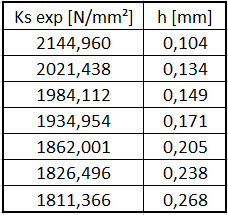
\includegraphics[width=0.3\linewidth]{Imagens/tabela ks1.png}
    \smallcaption{Fonte: Autor}
    \label{tab: parâmetros para ks_2}
 \end{table}

Após traçar o gráfico e ativar a linha de tendência, o próximo passo foi ver onde esta, ao estende-la, cruzava com o valor de $h$ igual a 1 e, assim achar a pressão específica de corte unitária, $Ks_1$. Os valores foram substituídos na equação da reta para verificação. O valor achado para o $Ks_1$ experimental foi de 1381,1 $N/mm^2$. E também pela linha de tendência, foi possível achar, através do coeficiente angular da reta, o valor de $z$, o qual foi 0,21025. Ambos os valores estão apresentados na Tabela (\ref{tab: ks1 e z exp}).

 \begin{table}[!htb]
 \centering
    \caption{$Ks_1$ e $z$ experimentais}
    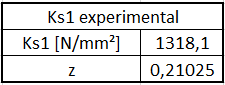
\includegraphics[width=0.3\linewidth]{Imagens/ks1 e z experiemnta.png}
    \smallcaption{Fonte: Autor}
    \label{tab: ks1 e z exp}
 \end{table}
 
Para fim de comparação foi necessário, através da literatura e tabelas normalizadas, achar os valores teóricos de $Ks_1$ e $z$. Portanto, como o aço utilizado no experimento foi o ABNT 1045, os valores achados foram de 1500 $N/mm^2$ e 0,22, respectivamente, como mostrados na Tabela (\ref{tab: Ks1 e z teo}). 
 
\begin{table}[!htb]
 \centering
    \caption{Valores de $Ks1$ e $z$ teóricos}
    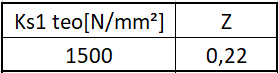
\includegraphics[width=0.3\linewidth]{Imagens/Ks1 e z tabelado.png}
    \smallcaption{Fonte: Autor}
    \label{tab: Ks1 e z teo}
 \end{table}

Com os valores de $Ks_1$ e $z$ teóricos achados foi possível calcular o valor de $F_c$ teórica através da relação de Kienzle (equação (\ref{eq: Relação de Kienzle})). Também foi possível calcular o valor de $Ks$ teórico, através da equação (\ref{eq: Pressão específica de corte}) e utilizando os dados de $A$ da Tabela (\ref{tab: Adicional}). Os resultados encontrados para a força e a pressão específica para cada experimento estão mostrados na Tabela (\ref{tab: Teoria}).


\begin{table}[!htb]
 \centering
    \caption{Cálculos teóricos}
    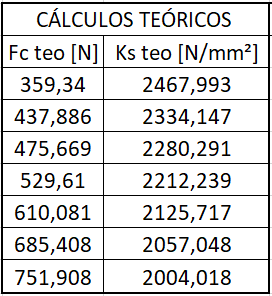
\includegraphics[width=0.3\linewidth]{Imagens/Calculos teoricos.png}
    \smallcaption{Fonte: Autor}
    \label{tab: Teoria}
 \end{table}

Com os resultados em mãos é observável que o parâmetro de corte que tem maior influência no cálculo do $Ks$ experimental é o avanço da ferramenta ($fn$). Isso porque, para a realização do levantamento do $Ks$ foi utilizado somente os sete primeiros ensaios, e, portanto, o avanço teve uma influência muito maior que os outros parâmetros no momento de calcular o valor da área, pois todos os valores de profundidade de corte foram iguais.

Pelos resultados, é possível verificar que os parâmetros de corte influenciam nos esforços de usinagem. Comparando, primeiro, somente a influência do avanço nas forças de usinagem é notável que ao aumentar o avanço ($f$) e manter os outros parâmetros ($a_p$ e $Vc$) constantes a força de corte ($F_c$), a força de avanço ($F_f$) e a força de penetração ($F_ap$) aumentam também. A Tabela (\ref{tab: avanço}) mostra esta influência nos sete primeiros ensaios, nos quais só foram alterados os avanços.

\begin{table}[!htb]
 \centering
    \caption{Comparação do avanço com as forças de usinagem}
    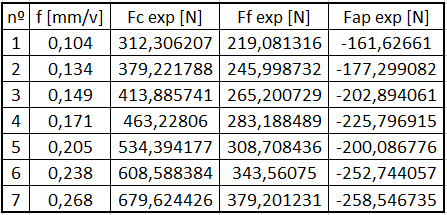
\includegraphics[width=0.5\linewidth]{Imagens/fxforças.png}
    \smallcaption{Fonte: Autor}
    \label{tab: avanço}
 \end{table}

A segunda comparação a ser feita é a influência da profundidade de corte ($a_p$) nos esforços de usinagem. Nos teste 8 à 11 somente as profundidades foram mudadas, mantendo a rotação em 450 $RPM$ e o avanço em 0,238 $mm/v$. Portanto, é possível observar pela Tabela (\ref{tab: profundidade}), que ao aumentar a profundidade de corte os esforços também aumentarão.

\begin{table}[!htb]
 \centering
    \caption{Comparação da profundidade de corte com as forças de usinagem}
    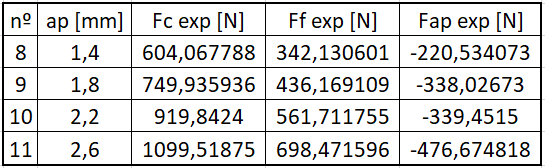
\includegraphics[width=0.6\linewidth]{Imagens/apxforças.png}
    \smallcaption{Fonte: Autor}
    \label{tab: profundidade}
 \end{table}

Uma outra comparação que se pode ser feita é sobre como a rotação ($n$) e a velocidade de corte ($Vc$) influenciam nestes esforços. Para isso, nos teste de 12 à 15, somente a rotação do torno foi alterada, mantendo o avanço e a profundidade de corte constantes em 0,205 $mm/v$ e 1,4 $mm$, respectivamente. Os resultados destas análises podem ser vistos na Tabela (\ref{tab: rotação}). Ao contrário dos outros parâmetros, a rotação e a velocidade de corte fazem com que os esforços sejam cada vez menores ao aumentar os seus respectivos valores.

\begin{table}[!htb]
 \centering
    \caption{Comparação da rotação com as forças de usinagem}
    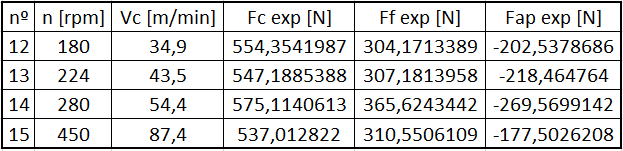
\includegraphics[width=0.7\linewidth]{Imagens/nvcxforças.png}
    \smallcaption{Fonte: Autor}
    \label{tab: rotação}
 \end{table}

O objetivo deste trabalho era achar o $Ks_1$ experimental e compará-lo com o teórico, através da relação de Kienzle, portanto a Tabela (\ref{tab: forçaks1}) mostra tal objetivo, utilizando o primeiro teste como base de comparação. É nítida a diferença do real com o teórico, porém é uma diferença já esperada, pois ao realizar experimentos há uma grande parcela de erros que podem acontecer durante os ensaios.

\begin{table}[!htb]
 \centering
    \caption{Comparação experimental com Kienzle}
    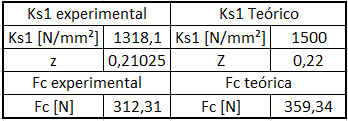
\includegraphics[width=0.5\linewidth]{Imagens/ks1txks1k.png}
    \smallcaption{Fonte: Autor}
    \label{tab: forçaks1}
 \end{table}
 
\section{Rugosidade}
Após a usinagem da barra nas diversas combinações dos parâmetros de usinagem, foram feitas as medições de rugosidade, para aferir qual parâmetro a afeta mais.

Começando pelo avanço da ferramenta, a Tabela (\ref{tab: Anvanço}), mostra os sete primeiros ensaios nos quais mudaram só os avanços. Foi possível observar que ao aumentar o valor do avanço a rugosidade do material também aumentou. Porém ocorreu um erro no primeiro ensaio, em que a rugosidade ficou maior que no segundo ensaio com um avanço maior. Este erro pode ter acontecido por diversas razões como erro ao posicionar a peça no rugosímetro, algum pode ter ficado cavaco preso na barra ou até mesmo por conta da geometria da ferramenta. 


\begin{table}[!htb]
 \centering
    \caption{Comparação do avanço com a rugosidade}
    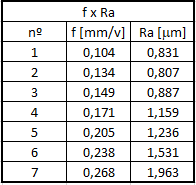
\includegraphics[width=0.3\linewidth]{Imagens/fxra.png}
    \smallcaption{Fonte: Autor}
    \label{tab: Anvanço}
 \end{table}

Seguindo com os ensaios e com as comparações, a profundidade de corte não tem uma influência muito significativa na rugosidade da peça, como visto na Tabela (\ref{tab: Profundidade}). Mas percebe-se que mesmo sendo pequena a diferença, quanto maior o valor da profundidade, maior a rugosidade da peça.Mas do mesmo modo que no primeiro ensaio, o ensaio de número 9 deu uma leve variada e as razões para isso podem ser as mesmas citadas para o outro ensaio.

\begin{table}[!htb]
 \centering
    \caption{Comparação da profundidade de corte com a rugosidade}
    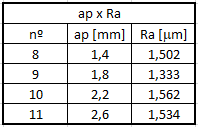
\includegraphics[width=0.3\linewidth]{Imagens/apxra.png}
    \smallcaption{Fonte: Autor}
    \label{tab: Profundidade}
 \end{table}

A velocidade de corte é o único do parâmetros observados que traz uma consequência diferente para a rugosidade. Comparando-os tem-se que com o aumento da velocidade e da rotação a rugosidade, nesse caso, diminui consideravelmente. A Tabela (\ref{tab: vcra}) mostra as relações encontradas para tal comparação.

\begin{table}[!htb]
 \centering
    \caption{Comparação da velocidade de corte com a rugosidade }
    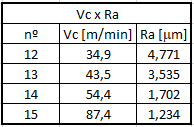
\includegraphics[width=0.3\linewidth]{Imagens/Vcxra2.png}
    \smallcaption{Fonte: Autor}
    \label{tab: vcra}
 \end{table}

 
 
\chapter{Conclusões}
Pode-se concluir que os parâmetros de corte de usinagem têm uma grande influência na rugosidade. Foi possível perceber que o incremento do valor do avanço resulta em um aumento da rugosidade, o incremento do valor da profundidade de corte não altera significativamente a rugosidade e a rotação, se aumentada, resulta em uma diminuição da rugosidade. Portanto, a superfície terá sua menor rugosidade quando a máquina tiver o menor avanço e a maior velocidade de corte.
Já para a pressão específica de corte foi possível notar que o valor experimental calculado foi um pouco menor que o encontrado na literatura e isto pode ter ocorrido por alguns erros e aproximações feitas nas medições durante a prática da experiência.

\printbibliography

\end{document}